% Options for packages loaded elsewhere
\PassOptionsToPackage{unicode}{hyperref}
\PassOptionsToPackage{hyphens}{url}
%
\documentclass[
  ignorenonframetext,
]{beamer}
\usepackage{pgfpages}
\setbeamertemplate{caption}[numbered]
\setbeamertemplate{caption label separator}{: }
\setbeamercolor{caption name}{fg=normal text.fg}
\beamertemplatenavigationsymbolsempty
% Prevent slide breaks in the middle of a paragraph
\widowpenalties 1 10000
\raggedbottom
\setbeamertemplate{part page}{
  \centering
  \begin{beamercolorbox}[sep=16pt,center]{part title}
    \usebeamerfont{part title}\insertpart\par
  \end{beamercolorbox}
}
\setbeamertemplate{section page}{
  \centering
  \begin{beamercolorbox}[sep=12pt,center]{part title}
    \usebeamerfont{section title}\insertsection\par
  \end{beamercolorbox}
}
\setbeamertemplate{subsection page}{
  \centering
  \begin{beamercolorbox}[sep=8pt,center]{part title}
    \usebeamerfont{subsection title}\insertsubsection\par
  \end{beamercolorbox}
}
\AtBeginPart{
  \frame{\partpage}
}
\AtBeginSection{
  \ifbibliography
  \else
    \frame{\sectionpage}
  \fi
}
\AtBeginSubsection{
  \frame{\subsectionpage}
}

\usepackage{amsmath,amssymb}
\usepackage{iftex}
\ifPDFTeX
  \usepackage[T1]{fontenc}
  \usepackage[utf8]{inputenc}
  \usepackage{textcomp} % provide euro and other symbols
\else % if luatex or xetex
  \usepackage{unicode-math}
  \defaultfontfeatures{Scale=MatchLowercase}
  \defaultfontfeatures[\rmfamily]{Ligatures=TeX,Scale=1}
\fi
\usepackage{lmodern}
\ifPDFTeX\else  
    % xetex/luatex font selection
\fi
% Use upquote if available, for straight quotes in verbatim environments
\IfFileExists{upquote.sty}{\usepackage{upquote}}{}
\IfFileExists{microtype.sty}{% use microtype if available
  \usepackage[]{microtype}
  \UseMicrotypeSet[protrusion]{basicmath} % disable protrusion for tt fonts
}{}
\makeatletter
\@ifundefined{KOMAClassName}{% if non-KOMA class
  \IfFileExists{parskip.sty}{%
    \usepackage{parskip}
  }{% else
    \setlength{\parindent}{0pt}
    \setlength{\parskip}{6pt plus 2pt minus 1pt}}
}{% if KOMA class
  \KOMAoptions{parskip=half}}
\makeatother
\usepackage{xcolor}
\newif\ifbibliography
\setlength{\emergencystretch}{3em} % prevent overfull lines
\setcounter{secnumdepth}{-\maxdimen} % remove section numbering

\usepackage{color}
\usepackage{fancyvrb}
\newcommand{\VerbBar}{|}
\newcommand{\VERB}{\Verb[commandchars=\\\{\}]}
\DefineVerbatimEnvironment{Highlighting}{Verbatim}{commandchars=\\\{\}}
% Add ',fontsize=\small' for more characters per line
\usepackage{framed}
\definecolor{shadecolor}{RGB}{241,243,245}
\newenvironment{Shaded}{\begin{snugshade}}{\end{snugshade}}
\newcommand{\AlertTok}[1]{\textcolor[rgb]{0.68,0.00,0.00}{#1}}
\newcommand{\AnnotationTok}[1]{\textcolor[rgb]{0.37,0.37,0.37}{#1}}
\newcommand{\AttributeTok}[1]{\textcolor[rgb]{0.40,0.45,0.13}{#1}}
\newcommand{\BaseNTok}[1]{\textcolor[rgb]{0.68,0.00,0.00}{#1}}
\newcommand{\BuiltInTok}[1]{\textcolor[rgb]{0.00,0.23,0.31}{#1}}
\newcommand{\CharTok}[1]{\textcolor[rgb]{0.13,0.47,0.30}{#1}}
\newcommand{\CommentTok}[1]{\textcolor[rgb]{0.37,0.37,0.37}{#1}}
\newcommand{\CommentVarTok}[1]{\textcolor[rgb]{0.37,0.37,0.37}{\textit{#1}}}
\newcommand{\ConstantTok}[1]{\textcolor[rgb]{0.56,0.35,0.01}{#1}}
\newcommand{\ControlFlowTok}[1]{\textcolor[rgb]{0.00,0.23,0.31}{#1}}
\newcommand{\DataTypeTok}[1]{\textcolor[rgb]{0.68,0.00,0.00}{#1}}
\newcommand{\DecValTok}[1]{\textcolor[rgb]{0.68,0.00,0.00}{#1}}
\newcommand{\DocumentationTok}[1]{\textcolor[rgb]{0.37,0.37,0.37}{\textit{#1}}}
\newcommand{\ErrorTok}[1]{\textcolor[rgb]{0.68,0.00,0.00}{#1}}
\newcommand{\ExtensionTok}[1]{\textcolor[rgb]{0.00,0.23,0.31}{#1}}
\newcommand{\FloatTok}[1]{\textcolor[rgb]{0.68,0.00,0.00}{#1}}
\newcommand{\FunctionTok}[1]{\textcolor[rgb]{0.28,0.35,0.67}{#1}}
\newcommand{\ImportTok}[1]{\textcolor[rgb]{0.00,0.46,0.62}{#1}}
\newcommand{\InformationTok}[1]{\textcolor[rgb]{0.37,0.37,0.37}{#1}}
\newcommand{\KeywordTok}[1]{\textcolor[rgb]{0.00,0.23,0.31}{#1}}
\newcommand{\NormalTok}[1]{\textcolor[rgb]{0.00,0.23,0.31}{#1}}
\newcommand{\OperatorTok}[1]{\textcolor[rgb]{0.37,0.37,0.37}{#1}}
\newcommand{\OtherTok}[1]{\textcolor[rgb]{0.00,0.23,0.31}{#1}}
\newcommand{\PreprocessorTok}[1]{\textcolor[rgb]{0.68,0.00,0.00}{#1}}
\newcommand{\RegionMarkerTok}[1]{\textcolor[rgb]{0.00,0.23,0.31}{#1}}
\newcommand{\SpecialCharTok}[1]{\textcolor[rgb]{0.37,0.37,0.37}{#1}}
\newcommand{\SpecialStringTok}[1]{\textcolor[rgb]{0.13,0.47,0.30}{#1}}
\newcommand{\StringTok}[1]{\textcolor[rgb]{0.13,0.47,0.30}{#1}}
\newcommand{\VariableTok}[1]{\textcolor[rgb]{0.07,0.07,0.07}{#1}}
\newcommand{\VerbatimStringTok}[1]{\textcolor[rgb]{0.13,0.47,0.30}{#1}}
\newcommand{\WarningTok}[1]{\textcolor[rgb]{0.37,0.37,0.37}{\textit{#1}}}

\providecommand{\tightlist}{%
  \setlength{\itemsep}{0pt}\setlength{\parskip}{0pt}}\usepackage{longtable,booktabs,array}
\usepackage{calc} % for calculating minipage widths
\usepackage{caption}
% Make caption package work with longtable
\makeatletter
\def\fnum@table{\tablename~\thetable}
\makeatother
\usepackage{graphicx}
\makeatletter
\def\maxwidth{\ifdim\Gin@nat@width>\linewidth\linewidth\else\Gin@nat@width\fi}
\def\maxheight{\ifdim\Gin@nat@height>\textheight\textheight\else\Gin@nat@height\fi}
\makeatother
% Scale images if necessary, so that they will not overflow the page
% margins by default, and it is still possible to overwrite the defaults
% using explicit options in \includegraphics[width, height, ...]{}
\setkeys{Gin}{width=\maxwidth,height=\maxheight,keepaspectratio}
% Set default figure placement to htbp
\makeatletter
\def\fps@figure{htbp}
\makeatother

\makeatletter
\@ifpackageloaded{tcolorbox}{}{\usepackage[skins,breakable]{tcolorbox}}
\@ifpackageloaded{fontawesome5}{}{\usepackage{fontawesome5}}
\definecolor{quarto-callout-color}{HTML}{909090}
\definecolor{quarto-callout-note-color}{HTML}{0758E5}
\definecolor{quarto-callout-important-color}{HTML}{CC1914}
\definecolor{quarto-callout-warning-color}{HTML}{EB9113}
\definecolor{quarto-callout-tip-color}{HTML}{00A047}
\definecolor{quarto-callout-caution-color}{HTML}{FC5300}
\definecolor{quarto-callout-color-frame}{HTML}{acacac}
\definecolor{quarto-callout-note-color-frame}{HTML}{4582ec}
\definecolor{quarto-callout-important-color-frame}{HTML}{d9534f}
\definecolor{quarto-callout-warning-color-frame}{HTML}{f0ad4e}
\definecolor{quarto-callout-tip-color-frame}{HTML}{02b875}
\definecolor{quarto-callout-caution-color-frame}{HTML}{fd7e14}
\makeatother
\makeatletter
\makeatother
\makeatletter
\makeatother
\makeatletter
\@ifpackageloaded{caption}{}{\usepackage{caption}}
\AtBeginDocument{%
\ifdefined\contentsname
  \renewcommand*\contentsname{Table of contents}
\else
  \newcommand\contentsname{Table of contents}
\fi
\ifdefined\listfigurename
  \renewcommand*\listfigurename{List of Figures}
\else
  \newcommand\listfigurename{List of Figures}
\fi
\ifdefined\listtablename
  \renewcommand*\listtablename{List of Tables}
\else
  \newcommand\listtablename{List of Tables}
\fi
\ifdefined\figurename
  \renewcommand*\figurename{Figure}
\else
  \newcommand\figurename{Figure}
\fi
\ifdefined\tablename
  \renewcommand*\tablename{Table}
\else
  \newcommand\tablename{Table}
\fi
}
\@ifpackageloaded{float}{}{\usepackage{float}}
\floatstyle{ruled}
\@ifundefined{c@chapter}{\newfloat{codelisting}{h}{lop}}{\newfloat{codelisting}{h}{lop}[chapter]}
\floatname{codelisting}{Listing}
\newcommand*\listoflistings{\listof{codelisting}{List of Listings}}
\makeatother
\makeatletter
\@ifpackageloaded{caption}{}{\usepackage{caption}}
\@ifpackageloaded{subcaption}{}{\usepackage{subcaption}}
\makeatother
\makeatletter
\@ifpackageloaded{tcolorbox}{}{\usepackage[skins,breakable]{tcolorbox}}
\makeatother
\makeatletter
\@ifundefined{shadecolor}{\definecolor{shadecolor}{rgb}{.97, .97, .97}}
\makeatother
\makeatletter
\makeatother
\makeatletter
\@ifpackageloaded{sidenotes}{}{\usepackage{sidenotes}}
\@ifpackageloaded{marginnote}{}{\usepackage{marginnote}}
\makeatother
\makeatletter
\makeatother
\ifLuaTeX
  \usepackage{selnolig}  % disable illegal ligatures
\fi
\IfFileExists{bookmark.sty}{\usepackage{bookmark}}{\usepackage{hyperref}}
\IfFileExists{xurl.sty}{\usepackage{xurl}}{} % add URL line breaks if available
\urlstyle{same} % disable monospaced font for URLs
\hypersetup{
  pdftitle={Network meta-analysis using survival data},
  pdfauthor={Nathan Green},
  hidelinks,
  pdfcreator={LaTeX via pandoc}}

\title{Network meta-analysis using survival data}
\author{Nathan Green}
\date{}
\institute{Department of Statistic Science \textbar{} University College
London}

\begin{document}
\frame{\titlepage}
\ifdefined\Shaded\renewenvironment{Shaded}{\begin{tcolorbox}[frame hidden, boxrule=0pt, enhanced, interior hidden, borderline west={3pt}{0pt}{shadecolor}, breakable, sharp corners]}{\end{tcolorbox}}\fi

\begin{frame}{Summary}
\protect\hypertarget{summary}{}
\begin{itemize}
\tightlist
\item
  Recap part one

  \begin{itemize}
  \tightlist
  \item
    Basic NMA with binary data
  \end{itemize}
\item
  NMA with survival data

  \begin{itemize}
  \tightlist
  \item
    IPD time to event
  \item
    Contrast-based data hazard ratios (HR)
  \end{itemize}
\item
  BUGS with R practical
\end{itemize}

\begin{tcolorbox}[enhanced jigsaw, toprule=.15mm, titlerule=0mm, colback=white, arc=.35mm, opacitybacktitle=0.6, coltitle=black, title={References}, breakable, toptitle=1mm, leftrule=.75mm, bottomtitle=1mm, rightrule=.15mm, opacityback=0, colframe=quarto-callout-note-color-frame, colbacktitle=quarto-callout-note-color!10!white, left=2mm, bottomrule=.15mm]

\begin{enumerate}
\item
  \textbf{Saramago P, Chuang LH, Soares MO}. \emph{Network meta-analysis
  of (individual patient) time to event data alongside (aggregate) count
  data}. BMC Med Res Methodol. 2014;14(1).
\item
  \textbf{Woods BS, Hawkins N, Scott DA}. \emph{Network meta-analysis on
  the log-hazard scale, combining count and hazard ratio statistics
  accounting for multi-arm trials: A tutorial}. BMC Med Res Methodol.
  2010;10.
\end{enumerate}

\end{tcolorbox}
\end{frame}

\begin{frame}{Recap of part 1}
\protect\hypertarget{recap-of-part-1}{}
\begin{itemize}
\tightlist
\item
  Unusual for a policy question to be informed by a single study

  \begin{itemize}
  \tightlist
  \item
    Must use all available and relevant evidence
  \end{itemize}
\end{itemize}

\begin{itemize}[<+->]
\item
  New treatment C: been trialled against old treatment B, but not to A
\item
  For health economic evaluation need to compare A/B/C together
\item
  Learn about C/A effect from C/B and B/A trial data
\item
  Also called ``mixed treatment comparisons''. Since can also ``mix''
  direct and indirect data on same comparison\ldots{}
\end{itemize}
\end{frame}

\begin{frame}{Count data equations}
\protect\hypertarget{count-data-equations}{}
\begin{tcolorbox}[enhanced jigsaw, toprule=.15mm, titlerule=0mm, colback=white, arc=.35mm, opacitybacktitle=0.6, coltitle=black, title={Fixed effects}, breakable, toptitle=1mm, leftrule=.75mm, bottomtitle=1mm, rightrule=.15mm, opacityback=0, colframe=quarto-callout-note-color-frame, colbacktitle=quarto-callout-note-color!10!white, left=2mm, bottomrule=.15mm]

\[
r_{st} \sim Bin(p_{st}, n_{st})\\
logit(p_{st}) = \mu_s + \delta_{st}\\
\delta_{st} \sim d_t - d_{t_{s0}}
\]

\end{tcolorbox}

\begin{tcolorbox}[enhanced jigsaw, toprule=.15mm, titlerule=0mm, colback=white, arc=.35mm, opacitybacktitle=0.6, coltitle=black, title={Random effects}, breakable, toptitle=1mm, leftrule=.75mm, bottomtitle=1mm, rightrule=.15mm, opacityback=0, colframe=quarto-callout-note-color-frame, colbacktitle=quarto-callout-note-color!10!white, left=2mm, bottomrule=.15mm]

\[
r_{st} \sim Bin(p_{st}, n_{st})\\
logit(p_{st}) = \mu_s + \delta_{st}\\
\delta_{st} \sim N(\mu^{\delta}_{st}, \sigma^2_{st})\\
\mu^{\delta}_{st} \sim d_t - d_{t_{s0}}
\]

\end{tcolorbox}
\end{frame}

\begin{frame}{More realistic situation}
\protect\hypertarget{more-realistic-situation}{}
\begin{itemize}
\tightlist
\item
  Different types of data we want to synthesise.
\end{itemize}
\end{frame}

\begin{frame}{Binary data with time to event data (TTE)}
\protect\hypertarget{binary-data-with-time-to-event-data-tte}{}
\begin{itemize}
\tightlist
\item
  Use example from Saramago (2014)\footnote<.->{\textbf{Saramago P,
    Chuang LH, Soares MO}. \emph{Network meta-analysis of (individual
    patient) time to event data alongside (aggregate) count data}. BMC
    Med Res Methodol. 2014;14(1).}
\end{itemize}

\pause

\begin{itemize}
\tightlist
\item
  The case study relates to compression systems aiming to deliver high
  compression to promote venous leg ulcer healing
\end{itemize}

\pause

\begin{itemize}
\tightlist
\item
  The final NMA contained data from 16 RCTs

  \begin{itemize}
  \tightlist
  \item
    2 included RCTs had full IPD data (841 participants) which included
    time to healing or censoring for each participant, together with
    other characteristics (treatment centre, ulcer duration, size,
    patient mobility).
  \item
    Remaining aggregate data only
  \end{itemize}
\end{itemize}

\marginnote{\begin{footnotesize}

\end{footnotesize}}
\end{frame}

\begin{frame}{Data}
\protect\hypertarget{data}{}
\begin{figure}

{\centering 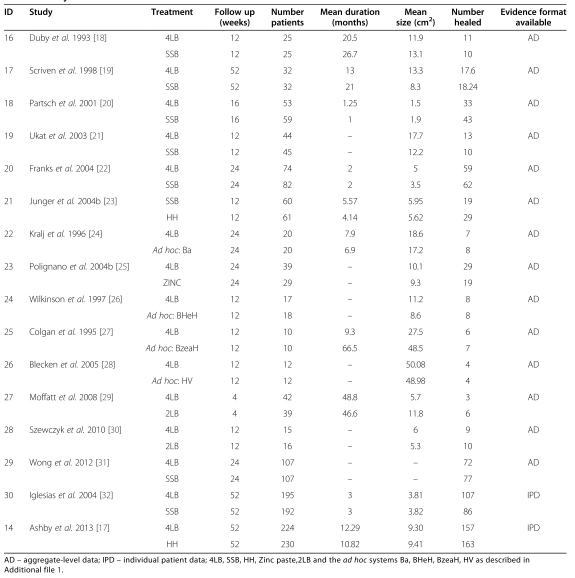
\includegraphics{paper-table.png}

}

\end{figure}
\end{frame}

\begin{frame}{Network diagram}
\protect\hypertarget{network-diagram}{}
\begin{figure}

{\centering 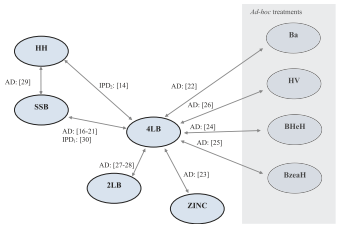
\includegraphics{paper-network-diagram.png}

}

\end{figure}
\end{frame}

\begin{frame}{IPD model}
\protect\hypertarget{ipd-model}{}
\begin{itemize}
\tightlist
\item
  \(i\)th participant in \(j\)th study in \(k\)th treatment arm
\end{itemize}

\[
t_{ijk} \sim Weibull(s, \lambda_{ijk}) I(t^c_{ijk})
\]

\[
\log(\lambda_{ijk}) = 
\begin{cases}
    \mu_j^{IPD} + \gamma_j^c + \beta_{0j}x_{ijk}, & \text{if } k=b\\
    \mu_j^{IPD} + d_{bk} + \gamma_j^c + \beta_{0j}x_{ijk}, & \text{if } k \gt b
\end{cases}
\]

\[
x_{ijk} \sim N(m,p) \;\;\; \gamma^c_j \sim N(0, \pi)
\]
\end{frame}

\begin{frame}{AD model}
\protect\hypertarget{ad-model}{}
\begin{itemize}
\tightlist
\item
  The linear predictor, \(\log(\lambda^{AD}_{jk})\) was a function of
  the baseline log-hazard of an event for treatment \(b\) in study
  \(j\), \(\mu^{AD}_{jb}\), and by the log-hazard ratio for treatment
  \(k\) and baseline treatment \(b\), \(d_{bk}\) (=
  \(d_{1k} − d_{1b}\)). Note that there are parameters common to both
  model parts, namely the log-hazard ratios and the shape parameter of
  the time to healing distribution.
\end{itemize}

\[
r_{jk} \sim Bin(p_{jk}, n_{nk})
\]

\[
p_{jk} = 1 - \exp(- \lambda_{jk}^{AD} {(t^{AD}_{jk})}^s)
\]

\[
\log(\lambda_{jk}^{AD}) =
\begin{cases}
    \mu_j^{AD}, & \text{if } k=b\\
    \mu_j^{AD} + d_{bk}, & \text{if } k \gt b
\end{cases}
\]
\end{frame}

\begin{frame}[fragile]{Data format}
\protect\hypertarget{data-format}{}
\begin{itemize}
\item
  \texttt{treat}: treatment arm (coded 1,2)
\item
  \texttt{baseline}: reference treatment code,
\item
  \texttt{t.obs}: time to event in months (under censoring)
\item
  \texttt{t.cens}: time of censoring in months,
\item
  \texttt{n.subjects}: Number of participants in IPD
\item
  \texttt{n.treat}: Number of treatments
\item
  \texttt{a.id} : study number
\item
  \texttt{a.treat} : treatment arm code (coded from 1 to number of
  treatments),
\item
  \texttt{r} : number of events in trial arm
\item
  \texttt{n} : number of patients in trial arm
\item
  \texttt{a.base} : reference treatment code
\item
  \texttt{a.time} : follow-up time of trial
\item
  \texttt{n.agg.trials} : Number of AD studies
\item
  \texttt{n.agg.arms} : Number of AD study arms
\end{itemize}
\end{frame}

\begin{frame}[fragile]{Data format}
\protect\hypertarget{data-format-1}{}
\begin{Shaded}
\begin{Highlighting}[]
\FunctionTok{load}\NormalTok{(here}\SpecialCharTok{::}\FunctionTok{here}\NormalTok{(}\StringTok{"part 2/practical/tte\_counts\_input\_data.RData"}\NormalTok{))}

\NormalTok{input\_dat}
\end{Highlighting}
\end{Shaded}

\begin{verbatim}
$n.subjects
[1] 3

$n.treat
[1] 2

$n.agg.trials
[1] 2

$n.agg.arms
[1] 2

$treat
[1] 1 1 2

$baseline
[1] 1 1 1

$t.obs
[1] 3.50 2.33   NA

$t.cens
[1]  0.0  0.0 11.9

$a.id
[1] 1 1 2

$a.treat
[1] 1 2 2

$r
[1] 11 10 10

$n
[1] 25 25 25

$a.base
[1] 1 1 1

$a.time
[1] 12 12 12
\end{verbatim}
\end{frame}

\begin{frame}[fragile]{Coding in BUGS}
\protect\hypertarget{coding-in-bugs}{}
\begin{itemize}
\tightlist
\item
  {Part 1}: Model for IPD
\end{itemize}

\begin{Shaded}
\begin{Highlighting}[numbers=left,,]
\NormalTok{model \{}
  \DocumentationTok{\#\#\# Part 1: Model for IPD}
  
  \ControlFlowTok{for}\NormalTok{(i }\ControlFlowTok{in} \DecValTok{1}\SpecialCharTok{:}\NormalTok{n.subjects) \{}
    \CommentTok{\# Weibull likelihood for IPD}
\NormalTok{    t.obs[i] }\SpecialCharTok{\textasciitilde{}} \FunctionTok{dexp}\NormalTok{(zu[i])}\FunctionTok{I}\NormalTok{(t.cens[i], )}
    
    \CommentTok{\# Model for IPD}
    \FunctionTok{log}\NormalTok{(zu[i]) }\OtherTok{\textless{}{-}}\NormalTok{ mu }\SpecialCharTok{+}\NormalTok{ d[treat[i]] }\SpecialCharTok{{-}}\NormalTok{ d[baseline[i]]}
\NormalTok{  \}}
  
  \CommentTok{\# Vague prior for IPD}
\NormalTok{  mu }\SpecialCharTok{\textasciitilde{}} \FunctionTok{dnorm}\NormalTok{(}\DecValTok{0}\NormalTok{, }\FloatTok{1.0E{-}6}\NormalTok{)}
\end{Highlighting}
\end{Shaded}
\end{frame}

\begin{frame}[fragile]{Coding in BUGS}
\protect\hypertarget{coding-in-bugs-1}{}
\begin{itemize}
\tightlist
\item
  {Part 2}: Model for aggregate data
\end{itemize}

\begin{Shaded}
\begin{Highlighting}[numbers=left,,]
  \DocumentationTok{\#\#\# Part 2: Model for aggregate data}
  
  \ControlFlowTok{for}\NormalTok{ (i }\ControlFlowTok{in} \DecValTok{1}\SpecialCharTok{:}\NormalTok{n.agg.arms) \{}
    \CommentTok{\# Binomial likelihood for AD}
\NormalTok{    r[i] }\SpecialCharTok{\textasciitilde{}} \FunctionTok{dbin}\NormalTok{(pa[i], n[i])}
    
    \CommentTok{\# Model for AD}
\NormalTok{    pa[i] }\OtherTok{\textless{}{-}} \DecValTok{1} \SpecialCharTok{{-}} \FunctionTok{exp}\NormalTok{(}\SpecialCharTok{{-}}\NormalTok{zu.a[i] }\SpecialCharTok{*}\NormalTok{ a.time[i])}
    \FunctionTok{log}\NormalTok{(zu.a[i]) }\OtherTok{\textless{}{-}}\NormalTok{ mu.a[a.id[i]] }\SpecialCharTok{+}\NormalTok{ d[a.treat[i]] }\SpecialCharTok{{-}}\NormalTok{ d[a.base[i]]}
\NormalTok{  \}}
  
  \CommentTok{\# Vague priors for AD}
  \ControlFlowTok{for}\NormalTok{(j }\ControlFlowTok{in} \DecValTok{1}\SpecialCharTok{:}\NormalTok{n.agg.trials) \{}
\NormalTok{    mu.a[j] }\SpecialCharTok{\textasciitilde{}} \FunctionTok{dnorm}\NormalTok{(}\DecValTok{0}\NormalTok{, }\FloatTok{1.0E{-}6}\NormalTok{)}
\NormalTok{  \}}
\end{Highlighting}
\end{Shaded}
\end{frame}

\begin{frame}[fragile]{Coding in BUGS}
\protect\hypertarget{coding-in-bugs-2}{}
\begin{itemize}
\tightlist
\item
  {Part 3}: Model for combining all estimates of treatment effect
\end{itemize}

\begin{Shaded}
\begin{Highlighting}[]
  \DocumentationTok{\#\#\# Model for combining all estimates of treatment effect}
  
  \CommentTok{\# Vague prior for basic parameters}
\NormalTok{  d[}\DecValTok{1}\NormalTok{] }\OtherTok{\textless{}{-}} \DecValTok{0}
  
  \ControlFlowTok{for}\NormalTok{ (k }\ControlFlowTok{in} \DecValTok{2}\SpecialCharTok{:}\NormalTok{n.treat) \{}
\NormalTok{    d[k] }\SpecialCharTok{\textasciitilde{}} \FunctionTok{dnorm}\NormalTok{(}\DecValTok{0}\NormalTok{, }\FloatTok{1.0E{-}6}\NormalTok{)}
\NormalTok{  \}}
\ErrorTok{\}}
\end{Highlighting}
\end{Shaded}
\end{frame}

\begin{frame}{Binary data with contrast-based survival data}
\protect\hypertarget{binary-data-with-contrast-based-survival-data}{}
\begin{itemize}
\tightlist
\item
  Use example from Woods (2010)\footnote<.->{\textbf{Woods BS, Hawkins
    N, Scott DA}. \emph{Network meta-analysis on the log-hazard scale,
    combining count and hazard ratio statistics accounting for multi-arm
    trials: A tutorial}. BMC Med Res Methodol. 2010;10.}
\end{itemize}

\pause

\begin{itemize}
\tightlist
\item
  Data on survival endpoints are usually summarised using either
  \emph{hazard ratio}, \emph{cumulative number of events}, or
  \emph{median} survival statistics
\end{itemize}

\pause

\begin{itemize}
\tightlist
\item
  NMA of survival endpoints can combine count and hazard ratio
  statistics in a single analysis on the hazard ratio scale
\end{itemize}

\pause

\begin{itemize}
\tightlist
\item
  A worked example of an analysis of mortality data in chronic
  obstructive pulmonary disease (COPD)
\end{itemize}

\marginnote{\begin{footnotesize}

\end{footnotesize}}
\end{frame}

\begin{frame}{Data}
\protect\hypertarget{data-1}{}
\begin{itemize}
\tightlist
\item
  Input RCT data binary counts table
\end{itemize}

\begin{figure}

{\centering 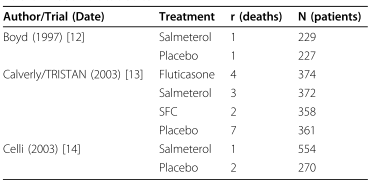
\includegraphics{woods-count-table.png}

}

\end{figure}

\begin{itemize}
\tightlist
\item
  Input RCT hazard summary table
\end{itemize}

\begin{figure}

{\centering 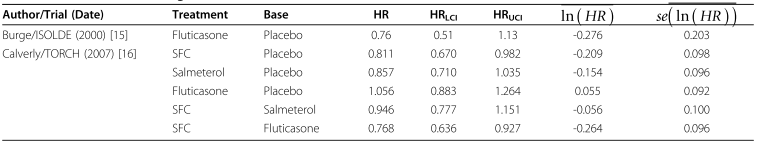
\includegraphics{woods-hr-table.png}

}

\end{figure}
\end{frame}

\begin{frame}{Count statistics on log-hazard ratio scale}
\protect\hypertarget{count-statistics-on-log-hazard-ratio-scale}{}
\begin{itemize}
\tightlist
\item
  For \(r_{sk}\) is the cumulative count of subject who have experienced
  an event in arm \(k\) of study \(s\); \(n_{sk}\) is total number of
  subjects in arm \(k\) of study \(s\) and \(F_{sk}\) is the cumulative
  probability of subject having an event.
\end{itemize}

\[
r_{sk} \sim Bin(F_{sk}, n_{sk})
\]

\begin{itemize}
\tightlist
\item
  The log cumulative hazard for each trial arm is then
\end{itemize}

\[
\ln(H_{sk}) = \ln(-\ln(1-F_{sk}))
\]

\begin{itemize}
\tightlist
\item
  The log cumulative hazard is estimated as the sum of a study specific
  `baseline' term \(\alpha_s\) and a treatment effect coefficient
  \(\beta_k\):
\end{itemize}

\[
\ln(H_{s,k}) = \alpha_s + \beta_k - \beta_b
\] where \(\beta_1 = 0\) for the reference treatment and \(\beta_b\)
represents the treatment effect for the baseline treatment in study
\(s\).
\end{frame}

\begin{frame}{What is \(\beta_k\)?}
\protect\hypertarget{what-is-beta_k}{}
\begin{itemize}
\tightlist
\item
  Under the assumption of proportional hazards, \(\beta_k\) is
  \emph{both} log cumulative hazard ratio \emph{and} log hazard ratio:
\end{itemize}

\[
\ln \left( \frac{\exp(\beta_k) h_{sb}}{h_{sb}} \right) = \ln \left( \frac{\int_0^t\exp(\beta_k) h_{sb}}{\int_0^th_{sb}} \right) = \beta_k
\]
\end{frame}

\begin{frame}{Combining count and hazard ratio statistics in an NMA}
\protect\hypertarget{combining-count-and-hazard-ratio-statistics-in-an-nma}{}
\begin{itemize}
\tightlist
\item
  \(x_{skb}\) is log hazard ratio estimate for study \(s\) comparing
  treatments \(k\) and \(b\)
\end{itemize}

\[
x_{skb} \sim N \left( \ln\left( \frac{h_{sk}}{h_{sb}} \right), se^2_{skb} \right)
\] then

\[
\ln\left( \frac{h_{sk}}{h_{sb}} \right) = \beta_k - \beta_b
\]
\end{frame}

\begin{frame}[fragile]{Coding in BUGS}
\protect\hypertarget{coding-in-bugs-3}{}
\begin{itemize}
\tightlist
\item
  For hazard ratio reporting studies
\end{itemize}

\begin{Shaded}
\begin{Highlighting}[]
\ControlFlowTok{for}\NormalTok{ (ii }\ControlFlowTok{in} \DecValTok{1}\SpecialCharTok{:}\NormalTok{LnObs) \{}
\NormalTok{  Lmu[ii] }\OtherTok{\textless{}{-}}\NormalTok{ alpha[Lstudy[ii]]}\SpecialCharTok{*}\NormalTok{multi[ii] }\SpecialCharTok{+}\NormalTok{ beta[Ltx[ii]] }\SpecialCharTok{{-}}\NormalTok{ beta[Lbase[ii]]}
\NormalTok{  Lprec[ii] }\OtherTok{\textless{}{-}} \DecValTok{1} \SpecialCharTok{/} \FunctionTok{pow}\NormalTok{(Lse[ii], }\DecValTok{2}\NormalTok{)}
\NormalTok{  Lmean[ii] }\SpecialCharTok{\textasciitilde{}} \FunctionTok{dnorm}\NormalTok{(Lmu[ii], Lprec[ii])}
\NormalTok{\}}
\end{Highlighting}
\end{Shaded}

\begin{itemize}
\tightlist
\item
  For binary data reporting studies
\end{itemize}

\begin{Shaded}
\begin{Highlighting}[]
\ControlFlowTok{for}\NormalTok{ (ss }\ControlFlowTok{in} \DecValTok{1}\SpecialCharTok{:}\NormalTok{BnObs) \{}
\NormalTok{  logCumHaz[ss] }\OtherTok{\textless{}{-}}\NormalTok{ alpha[Bstudy[ss]] }\SpecialCharTok{+}\NormalTok{ beta[Btx[ss]] }\SpecialCharTok{{-}}\NormalTok{ beta[Bbase[ss]]}
\NormalTok{  cumFail[ss] }\OtherTok{\textless{}{-}} \DecValTok{1} \SpecialCharTok{{-}} \FunctionTok{exp}\NormalTok{(}\SpecialCharTok{{-}}\DecValTok{1} \SpecialCharTok{*} \FunctionTok{exp}\NormalTok{(logCumHaz[ss]))}
\NormalTok{  Br[ss] }\SpecialCharTok{\textasciitilde{}} \FunctionTok{dbin}\NormalTok{(cumFail[ss], Bn[ss])}
\NormalTok{  \}}
\end{Highlighting}
\end{Shaded}
\end{frame}

\begin{frame}{Going further}
\protect\hypertarget{going-further}{}
\begin{tcolorbox}[enhanced jigsaw, toprule=.15mm, titlerule=0mm, colback=white, arc=.35mm, opacitybacktitle=0.6, coltitle=black, title={References}, breakable, toptitle=1mm, leftrule=.75mm, bottomtitle=1mm, rightrule=.15mm, opacityback=0, colframe=quarto-callout-note-color-frame, colbacktitle=quarto-callout-note-color!10!white, left=2mm, bottomrule=.15mm]

\begin{enumerate}
\item
  \textbf{Saramago P, Chuang LH, Soares MO}. \emph{Network meta-analysis
  of (individual patient) time to event data alongside (aggregate) count
  data}. BMC Med Res Methodol. 2014;14(1).
\item
  \textbf{Woods BS, Hawkins N, Scott DA}. \emph{Network meta-analysis on
  the log-hazard scale, combining count and hazard ratio statistics
  accounting for multi-arm trials: A tutorial}. BMC Med Res Methodol.
  2010;10.
\item
  \textbf{Donegan S, Williamson P, D'Alessandro U, Garner P, Smith C}:
  \emph{Combining individual patient data and aggregate data in mixed
  treatment comparison meta-analysis: individual patient data may be
  beneficial if only for a subset of trials}. Stat Med 2013,
  32(6):914--930.
\item
  \textbf{Berlin J, Santanna J, Schmid C, Szczech L, Feldman H}:
  \emph{Individual patient- versus group-level data meta-regressions for
  the investigation of treatment effect modifiers: ecological bias rears
  its ugly head}. Stat Med 2002, 21(3):371--387.
\item
  \textbf{Riley R, Lambert P, Staessen J, Wang J, Gueyffier F, Thijs L,
  Boutitie F}: \emph{Meta-analysis of continuous outcomes combining
  individual patient data and aggregate data}. Stat Med 2008,
  27(11):1870--1893
\end{enumerate}

\end{tcolorbox}
\end{frame}



\end{document}
